\chapter{Ice Reservoirs}

\section{Introduction}

\begin{figure}[t]
\centering
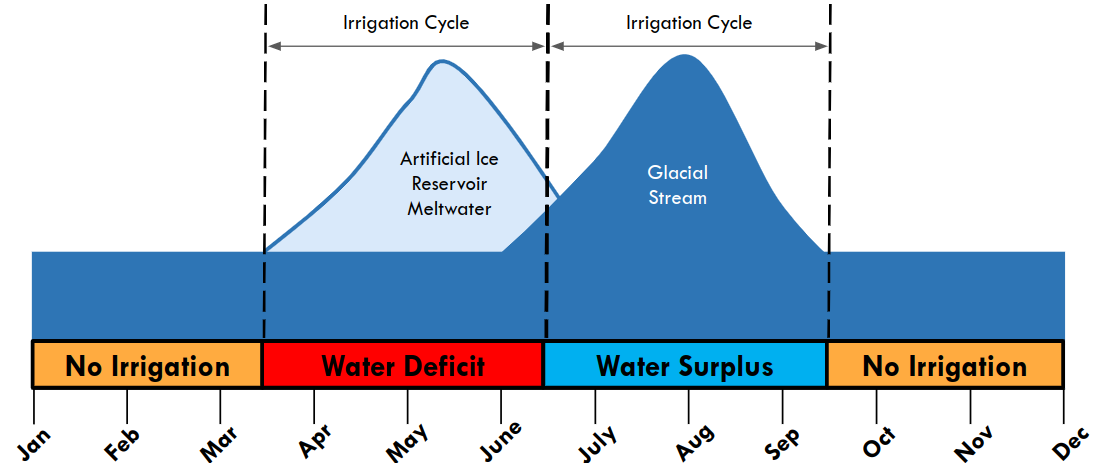
\includegraphics[width=12cm]{Figures/irrigation_cycles.png}

\caption{Seasonal variation in the availability of irrigation water. The graph highlights the crucial role of
AIRs in bridging the phase of water scarcity in spring. Adapted from: \cite{nusserLocalKnowledgeGlobal2016}}

\label{fig:irrigation_cycles}
\end{figure}

Cryosphere-fed irrigation networks in arid mountain regions are completely dependent on timely availability of
meltwater from glaciers, snow and permafrost \citep{immerzeelImportanceVulnerabilityWorld2020,
farhanHydrologicalRegimesConjunction2015, tveitenGlacierGrowingLocal2007}. With the accelerated decline of
glaciers due to climate change \citep{nusserLocalKnowledgeGlobal2016}, these regions are experiencing water
scarcity particularly during the spring season \citep{norphelSnowWaterHarvesting2015,
mukhopadhyayReevaluationSnowmeltGlacial2015} (see Fig. \ref{fig:irrigation_cycles}). This seasonal water
scarcity makes it essential to provide supplementary irrigation in order to sustain agricultural output and take
advantage of the complete growing season \citep{nusserLocalKnowledgeGlobal2016, vincentEnergyClimateChange2009}.

To cope with this recurrent water scarcity, villagers in the region of Ladakh have developed two types of
artificial ice reservoirs (AIRs): ice stupas and ice terraces.  All these types of ice reservoirs capture water
in the autumn and winter, allowing it to freeze, and hold it until spring, when it melts and flows down to
fields \citep{ipccChapterHighMountain2019, vinceGlacierMan2009, clouseLadakhArtificialGlaciers2017,
nusserSociohydrologyArtificialGlaciers2019}. In this way, they retain a previously unused portion of the annual
flow and facilitate its use to supplement the decreased flow in the following spring (see Fig.
\ref{fig:irrigation_cycles}). This study focuses on the form of AIRs locally called as ice stupas.

Over the past decade, several ice stupas have been built to supplement irrigation water supply of mountain
villages in India \citep{wangchukIceStupaCompetition2020, palmerStoringFrozenWater2022,
aggarwalAdaptationClimateChange2021}, Kyrgyzstan \citep{bbcnewsBrightArtificialGlacier2020} and Chile
\citep{reutersConservationistsChileAim2021}. Despite this widespread adoption, only a few publications examine
the role of AIRs in the water resource management of these regions. None of these publications study AIRs
outside Ladakh. Moreover, the published quantifications of the water storage capacity of AIRs just in Ladakh
also vary widely between these studies \citep{norphelSnowWaterHarvesting2015, baglaArtificialGlaciersHelp1998}.
This thesis is a contribution to close this knowledge gap.

Quantifying the water storage capacity of AIRs is not straightforward. It requires an understanding of the
response of these AIRs both to meteorological conditions and construction strategies used. Since AIRs are ice
structures with similar surface processes like glaciers, glacier models could be used to quantify meteorological
influences. However, due to their limited size, and comparatively more variable surface area, this assessment
requires a modelling approach which is optimally constrained with comprehensive data from in-situ field
measurements. Moreover, a spirit of improvisation guides the design and construction of AIRs making it difficult
to make quantitative comparison from site to site. Therefore, the influence of the different construction
strategies used also have to be captured in this modelling approach. 

This thesis fulfills these requirements as it provides a new set of AIR-specific volume and area measurements
from drone flights along with meteorological data during the construction period. All these datasets were
produced through construction strategies using fountain systems that are quantified via in-situ observations of
the fountain characteristics and discharge rate measurements. This thesis also provides a one-dimensional AIR
model which is calibrated and validated with several AIR datasets from locations with different meteorological
conditions and different fountain systems.


\section{Objectives}

The main objective of this thesis is to quantify the water storage potential of AIRs based on the construction
site and fountain chosen. 

An integrated study approach including field measurements and modelling is applied to
answer the following research questions: 

\begin{itemize}

\item What is the influence of construction location and fountain characteristics on AIR volume evolution? 

\item How can ice stupa fountain systems be engineered to reduce water loss and maintenance of AIRs?

\end{itemize}

An energy and mass balance model for artificial ice reservoirs was set up to answer the first research question
(paper I and II). Since in-situ measurements were required to run this model, a measurement campaign was
executed in Switzerland and India during the past 4 winters. These datasets provided the necessary input,
calibration and validation data to model the evolution of AIRs and study their sensitivity to meteorological
conditions (paper II). 

A weather-sensitive construction strategy was developed to answer the second research question. This
construction strategy employed fountains whose discharge rate was regulated by automation system using the AIR
model developed before. This weather-sensitive construction strategy was compared with the traditional
construction strategy to quantify its advantages and disadvantages (paper III).

\section{Structure}

Chapter 1 introduces the motivation of this work and provides a summary of the state of knowledge about AIRs
prior to this thesis. Chapter 2 describes the origins of this technology as a religious practice. Chapter 3
gives an overview about the study sites and introduces the different field techniques applied. The influence of
the construction location through its meteorological and topographical conditions are presented in Chapter 4.
The engineering design of AIR technologies are showcased in Chapter 5 along with suggestions for their
improvement. Chapter 6 concludes the thesis with a synthesis and future outlook. Papers I, II and III are
included in the Appendix.


